\documentclass[12pt,a4paper]{report}
\usepackage[italian]{babel}
%\usepackage[T1]{fontenc} % Riga da commentare se si compila con PDFLaTeX
\usepackage{geometry}
\usepackage{graphicx}
\usepackage{hyperref}
\usepackage[utf8]{inputenc}
\usepackage{lipsum} % genera testo fittizio
\usepackage[nottoc,numbib]{tocbibind}
\usepackage{titlesec}
\usepackage{cochineal}
\usepackage[cochineal]{newtxmath}
\usepackage[simplified]{pgf-umlcd}
\usepackage{float}
\usepackage{wrapfig,lipsum}
\usepackage{fancyhdr, etoolbox}
\usepackage{xcolor}
\usepackage{listings}
\usepackage{xparse}
\usepackage{booktabs}
\usepackage{url}
\usepackage{setspace}
\usepackage{longtable}
\usepackage{etaremune}
\usepackage{subfig}
\usepackage[edges]{forest}
\usepackage{matlab-prettifier}

\NewDocumentCommand{\codeword}{v}{%
    \texttt{\textcolor{blue}{#1}}%
}

\lstset{language=C,keywordstyle={\bfseries \color{blue}}}

%\usetikzlibrary{calc}
\pagestyle{fancy}

\fancyhead{}
\fancyhead[OL]{\ifnumodd{\value{page}}{\slshape \leftmark}{\slshape SEZIONE \rightmark}}
\fancypagestyle{mystyle}{
    \fancyhead[OL]{\slshape \leftmark}
}
\fancyfoot[C]{\thepage}

\fontfamily{bch}\selectfont


\definecolor{darkgray}{rgb}{.4,.4,.4}
\definecolor{purple}{rgb}{0.65, 0.12, 0.82}

\definecolor{pblue}{rgb}{0.13,0.13,1}
\definecolor{pgreen}{rgb}{0,0.5,0}
\definecolor{pred}{rgb}{0.9,0,0}
\definecolor{pgrey}{rgb}{0.46,0.45,0.48}

\usepackage{listings}
\lstset{language=Java,
  showspaces=false,
  showtabs=false,
  breaklines=true,
  tabsize=1,
  showstringspaces=false,
  breakatwhitespace=true,
  commentstyle=\color{pgreen},
  keywordstyle=\color{pblue},
  stringstyle=\color{pred},
  basicstyle=\ttfamily,
  moredelim=[il][\textcolor{pgrey}]{$$},
  moredelim=[is][\textcolor{pgrey}]{\%\%}{\%\%}
}

\newcommand{\norm}[1]{\left\lVert#1\right\rVert}
\newcommand{\normtwo}[1]{\left\lVert#1\right\rVert _2^2}
\newcommand{\nukenorm}[1]{\left\lVert#1\right\rVert _*}
\newcommand{\frobnorm}[1]{\left\lVert#1\right\rVert _F}
\newcommand{\R}{\mathbb{R}}
\newcommand{\ux}{\underline{x}}
\newcommand{\uy}{\underline{y}}
\newcommand{\ug}{\underline{g}}
\newcommand{\ue}{\underline{e}}
\newcommand{\uk}{\underline{k}}
\newcommand{\uw}{\underline{w}}
\newcommand{\uv}{\underline{v}}
\newcommand{\ub}{\underline{b}}
\newcommand{\uc}{\underline{c}}
\newcommand{\uone}{\underline{1}}
\newcommand{\ut}{\underline{\theta}}
\newcommand{\est}{\underline{\hat{\theta}}}

\newcommand{\mF}{\mathcal{F}}
\newcommand{\mS}{\mathcal{S}}


\titleformat{\chapter}[display]{\Huge\bfseries}{}{0pt}{\thechapter.\ }

\graphicspath{{figures/}}
%
%\addtolength{\topmargin}{-.875in} % reduce the default top margin
%\addtolength{\topmargin}{-2cm} % reduce the default top margin
%

\tolerance=1
\emergencystretch=\maxdimen
\hyphenpenalty=10000
\hbadness=10000

%%%%%%%%%%%%%%%%%%%%%%%%%%%%%%%%%%
%                                %
%     Begin Docuemnt [start]     %
%                                %
%%%%%%%%%%%%%%%%%%%%%%%%%%%%%%%%%%
\begin{document}

\begin{titlepage}

%%%%%%%%%%%%%%%%%%%%%%%%%%%%%%
%     Title Page [start]     %
%%%%%%%%%%%%%%%%%%%%%%%%%%%%%%
% Declare new goemetry for the title page only.
{\Large \noindent Paolo Speziali} \newline

\vspace{1cm}

{\begin{flushleft}

  {\normalsize \noindent Tesina di}
  \vspace{0.2cm}
  
  {\Large \noindent Signal Processing and Optimization for Big Data}

  \vspace{0.2cm}
  
  {\large \noindent del Prof.~Paolo Banelli}

  \vspace{2cm}

  \fontsize{21.8}{26.16} \selectfont \bfseries \noindent 
  Low-Rank Matrix Completion \\
  con implementazione e \\ 
  verifica sperimentale \\
  \end{flushleft}}
  
  \vspace{4cm}


\noindent Perugia, Anno Accademico 2022/2023

\noindent Università degli Studi di Perugia \\
Corso di laurea magistrale in Ingegneria Informatica e Robotica \\
Curriculum Data Science \\
Dipartimento di Ingegneria

\vspace{0.7cm}

\noindent 
\includegraphics[width=0.5\textwidth]{Figures/logounipg2021}
% Ends the declared geometry for the titlepage
\restoregeometry
\end{titlepage}
\normalfont
%%%%%%%%%%%%%%%%%%%%%%%%%%%%
%     Title Page [end]     %
%%%%%%%%%%%%%%%%%%%%%%%%%%%%
\newpage \thispagestyle{empty} \ \newpage
%%%%%%%%%%%%%%%%%%%%%%%%%%
%     Indice [start]     %
%%%%%%%%%%%%%%%%%%%%%%%%%%
\onehalfspacing
\tableofcontents

%%%%%%%%%%%%%%%%%%%%%%%%
%     Indice [end]     %
%%%%%%%%%%%%%%%%%%%%%%%%

\chapter{Introduzione}

Lo scopo di questa tesina è l'implementazione in ambiente MATLAB di alcuni algoritmi
atti a risolvere il problema dello stimare i valori mancanti di una matrice di cui
abbiamo a disoposizione solo un sottoinsieme limtato di entry.

{\let\clearpage\relax\chapter{Concetti teorici}}

\section{Formulazione del problema}

Sia $M\in\mathbb{R}^{n_1\times n_2}$ con rango $r$, e sia data la sua scomposizione ai valori
singolari (SVD):
$$M=U\Sigma V^T \quad\text{con}\quad U\in\mathbb{R}^{n_1\times r},
\;\Sigma\in\mathbb{R}^{r\times r},\;V\in\mathbb{R}^{n_2\times r}$$
dove $U$ e $V$ sono composte da colonne ortonormali, e $\Sigma$ è una matrice
diagonale con i valori singolari ordinati in modo non crescente
($\sigma_1\geq\sigma_2\geq\ldots\geq\sigma_r>0$).

I \textbf{gradi di libertà} di $M$ sono $(n_1 + n_2 - r)r$, che è il numero totale di parametri
necessari per specificare univocamente la matrice $M$.

\newpage

Supponiamo di avere delle osservazioni parziali di $M$ su un insieme di indici
$$\Omega \subset \{1,2,\ldots,n_1\}\times\{1,2,\ldots,n_2\}$$
e definiamo l'\textbf{operatore di osservazione}
$\mathcal{P}_{\Omega}:\mathbb{R}^{n_1\times n_2}\to\mathbb{R}^{n_1\times n_2}$ come segue:
$$\left[\mathcal{P}_{\Omega}(M)\right] _{ij}=\left\{\begin{matrix}M_{ij}, & \text{se}\; (i,j)\in X \\ 0, & \text{altrimenti}\end{matrix}\right.$$
Il nostro obiettivo è recuperare $M$ da $\mathcal{P}_{\Omega}(M)$
quando il numero di osservazioni\\ $m = |\Omega| \ll n_1 n_2$, ovvero quando
è molto più piccolo del numero di elementi in $M$, e sotto l'assunzione che $M$
sia a basso rango, ovvero $r\ll\min(n_1,n_2)$.
Per semplicità notazionale, poniamo $n=\max(n_1,n_2)$.

\section{Soluzione del problema}

Quali tipi di matrici a basso rango possiamo completare?
Consideriamo le matrici $M_1$ e $M_2$ di rango $1$ e di dimensione $4 \times 4$:

$$M_1 = \begin{bmatrix}
  1 & 0 & 0 & 0 \\ 1 & 0 & 0 & 0 \\ 1 & 0 & 0 & 0 \\ 1 & 0 & 0 & 0
\end{bmatrix}
\qquad
M_2 = \begin{bmatrix}
  1 & 1 & 1 & 1 \\ 1 & 1 & 1 & 1 \\ 1 & 1 & 1 & 1 \\ 1 & 1 & 1 & 1
\end{bmatrix}$$

La matrice $M_1$ è più difficile da completare
poiché la maggior parte delle sue voci sono nulle
e quindi abbiamo bisogno di raccogliere più misure per assicurarsi
che abbastanza ``massa'' venga dalle sue voci non nulle.
Al contrario, la massa di $M_2$ è distribuita più uniformemente su tutte le voci,
rendendolo più facile da propagare da una voce all'altra.

In altre parole, una matrice a basso rango è più facile da completare se la sua energia
si distribuisce uniformemente su diverse coordinate.
Questa proprietà è catturata dalla \textbf{coerenza}, che misura l'allineamento
tra lo spazio delle colonne/righe della matrice a basso rango con i vettori della base standard.

Per una matrice $U\in\mathbb{R}^{n_1\times r}$ con colonne ortonormali,
$P_U$ rappresenta la proiezione ortogonale sullo spazio delle colonne di $U$.
La \textbf{coerenza} di $U$ è definita come segue:
$$ \mu(U) = \frac{n_1}{r}\, \underset{1 \leq i \leq n_1}{max}\, \normtwo{P_U\, \underline{e}_i}
= \frac{n_1}{r}\, \underset{1 \leq i \leq n_1}{max}\, \normtwo{U^T\, \underline{e}_i}$$
dove $\underline{e}_i$ è l'$i$-esimo vettore della base canonica.

Per una matrice a basso rango $M$ il cui SVD è data da $M=U\Sigma V^T$,
la coerenza di $M$ è definita come:

$$ \mu = max\{\mu(U), \mu(V)\} $$

Si noti che la coerenza $\mu$ è determinata dai vettori singolari di $M$ ed
è indipendente dai suoi valori singolari.

Poiché $1\leq \mu(U) \leq \frac{n_1}{r}$
e $1\leq \mu(V) \leq \frac{n_2}{r}$, abbiamo $1\leq \mu \leq \frac{n}{r}$.
Nell'esempio precedente, la coerenza di $M_1$ coincide con il limite superiore
$\frac{n}{r}$, mentre quella di $M_2$ coincide con il limite inferiore $1$.
Più $\mu$ è piccolo, più è facile completare la matrice.

Possiamo incontrare alcune matrici la cui ricostruzione non è possibile,
un esempio sarebbe una matrice con tutti i valori eccetto quelli di una colonna completamente
mancante, essa non potrà essere recuperata in quanto potrebbe giacere ovunque nello
spazio delle colonne della matrice.
Ci servono quindi almeno $r$ osservazioni per colonna/riga.

Per evitare di incorrere in questi casi sfavorevoli, supponiamo di star utilizzando
un pattern di osservazione causale che segua un modello di distribuzione di probabilità
noto come \textbf{Bernoulli}, per cui ogni valore viene osservato indipendentemente
e con probabilità uguale a $p := \frac{m}{n_1\cdot n_2}$.

Non è possibile recuperare una matrice a basso rango con un numero di osservazioni
ad uno dell'ordine di $O(\mu n r \log n)$ utilizzando un qualsiasi algoritmo,
questo è noto come l'\textbf{information-theoretic lower bound}.
Rispetto ai gradi di libertà, che sono dell'ordine di $nr$,
paghiamo un prezzo in complessità di campionamento di un fattore $\mu \log n$,
mettendo ancora una volta in evidenza il ruolo della coerenza nel completamento di matrici a basso rango.

\newpage

\subsection{Completamento di matrici tramite ottimizzazione convessa}

Cercando di sfruttare la struttura a basso rango della soluzione, un'euristica naturale
è trovare la matrice con rango minore che permette tali osservazioni:
$$ \underset{\Phi \in \mathbb{R}^{n_1 \times n_2}}{min}\;\; rank(\Phi) $$
$$ s.t. \;\;  \mathcal{P}_{\Omega}(\Phi) = \mathcal{P}_{\Omega}(M) $$ 
Tuttavia, essendo la minimizzazione del rango un problema NP-arduo,
tale formulazione è intrattabile, possiamo però
pensare a un possibile rilassamento di questa euristica.

Notando che il rango di $\Phi$ è uguale al numero dei suoi valori singolari non nulli,
sostituiamo $rank(\Phi)$ con la somma dei suoi valori singolari, indicata come \textbf{nuclear norm}:
$$ \nukenorm{\Phi} \triangleq \sum_{i=1}^n \sigma_i(\Phi) $$
Quindi, invece di risolvere direttamente il problema visto precedentemente,
risolviamo la minimizzazione della nuclear norm, che cerca una matrice con la nuclear norm
minima che soddisfa tutte le misurazioni:
$$ \underset{\Phi \in \mathbb{R}^{n_1 \times n_2}}{min}\;\; \nukenorm{\Phi} $$
$$ s.t. \;\;  \mathcal{P}_{\Omega}(\Phi) = \mathcal{P}_{\Omega}(M) $$ 
Si ottiene così un programma convesso che può
essere risolto in modo efficiente in tempo polinomiale.
Inoltre, non richiede la conoscenza
del rango a priori.

La minimizzazione della nuclear norm può recuperare esattamente
una matrice di basso rango non appena il numero di misurazioni è leggermente più grande
dell'information-theoretic lower bound di un fattore logaritmico.
Supponiamo che ogni valore della matrice $M$ venga osservato indipendentemente
con una probabilità $p \in (0,1)$. Se:
$$ p \leq C \; \frac{\mu r \log^2 n}{n} $$
per una qualche $C>0$ abbastanza grande, allora con grande probabilità
l'algoritmo recupera esattamente 
la matrice $M$ come soluzione ottima.

\subsection{Completamento di matrici tramite ottimizzazione non convessa}

L'algoritmo appena visto può essere particolarmente costoso in termini di tempo e memoria
per problemi su larga scala a causa del dover ottimizzare e memorizzare la variabile $\Phi$.
Pertanto, è necessario considerare approcci alternativi che scalino in modo più favorevole con $n$.
Ciò porta al secondo algoritmo basato su gradient descent utilizzando un'inizializzazione adeguata.

Se il rango della matrice $M$ è noto, è naturale incorporare questa conoscenza 
e considerare un problema least-square vincolato al rango:
$$ \underset{\Phi \in \mathbb{R}^{n_1 \times n_2}}{min}\;\; \frobnorm{\mathcal{P}_{\Omega}(\Phi - M)}^2 $$
$$ s.t. \;\;  rank(\Phi) \leq r $$ 
dove $\frobnorm{\cdot}$ è la \textbf{Frobenius norm} di una matrice.
Utilizzando la fattorizzazione a basso rango $\Phi = XY^T$ dove $X \in \mathbb{R}^{n_1 \times r}$
e $Y \in \mathbb{R}^{n_2 \times r}$, riscriviamo il problema qui sopra come 
un problema d'ottimizzazione non vincolato e non convesso:
$$ \underset{X,Y}{min}\;\; \mathit{f}(X,Y) := \frobnorm{\mathcal{P}_{\Omega}(XY^T - M)}^2 $$
Le complessità a livello di memoria di $X$ e $Y$ sono lineari in $n$.
Introduciamo una loss function modificata per sistemare alcuni
problemi di scalabilità e avere norme bilanciate:
$$ F(X,Y) = \frac{1}{4p}\mathit{f}(X,Y) + \frac{1}{16}\frobnorm{X^TX - Y^TY}^2  $$
$$ = \frac{1}{4p}\frobnorm{\mathcal{P}_{\Omega}(XY^T - M)}^2 + \frac{1}{16}\frobnorm{X^TX - Y^TY}^2 $$
I cui gradienti rispetto a $X$ e a $Y$ sono:
$$ \frac{\partial F(X,Y)}{\partial X} = \frac{1}{4p} ((\mathcal{P}_{\Omega}(XY^T - M))Y) + \frac{1}{8} X (X^TX-Y^TY)$$
$$ \frac{\partial F(X,Y)}{\partial Y} = \frac{1}{4p} (X^T(\mathcal{P}_{\Omega}(XY^T - M)))^T + \frac{1}{8} Y (X^TX-Y^TY)$$
\newpage
La probabilità $p$ delle osservazioni può essere stimata com $p = \frac{|\Omega|}{n_1\cdot n_2}$.

Ma come facciamo a ottimizzare la loss non convessa $F(X,Y)$?
\begin{enumerate}
  \item Troviamo un'inizializzazione ``spettrale" che sia vicina alla verità di base.
  Consideriamo la matrice parzialmente osservata $\frac{1}{p}\,\mathcal{P}_{\Omega}(M)$,
  che è una stima non polarizzata di $M$ con valore atteso pari a
  $E[\frac{1}{p}\,\mathcal{P}_{\Omega}(M)] = M$.
  Perciò, un'approssimazione best rank-$r$ produce una stima iniziale adeguata.

  Sia tale approssimazione $U_0 \Sigma_0 V_0^T$, inizializzeremo con:
  $$ X_0 = U_0 \Sigma_0^{1/2} \;\; \text{ e } \;\; Y_0 = V_0 \Sigma_0^{1/2} $$
  \item Raffiniamo la stima iniziale con semplici metodi iterativi secondo la
  seguente regola d'aggiornamento:
  $$ \begin{bmatrix}
    X_{t+1}\\ 
    Y_{t+1}
    \end{bmatrix}
    =
    \begin{bmatrix}
    X_{t}\\ 
    Y_{t}
    \end{bmatrix}
    - \eta_t
    \begin{bmatrix}
    \nabla_X \, F(X_t, Y_t)\\ 
    \nabla_Y \, F(X_t, Y_t)
  \end{bmatrix} $$
  dove $\eta_t$ è la step-size.
\end{enumerate}
Data la costante $\kappa = \sigma_1/\sigma_r$,
se la step-size $0 < \eta_t \equiv \eta \leq 2 / (25\cdot\kappa\cdot\sigma_1)$
e se il numero di osservazioni è dell'ordine di $\mu^3 r^3 n \log^3 n$,
perciò se:
$$ p \leq C \; \frac{\mu^3 r^3 n \log^3}{n} $$
per una qualche $C>0$ abbastanza grande,
il gradient descent converge ad una velocità geometrica.
Il numero di iterazioni è indipendente dalla grandezza del problema e quindi
il costo computazionale è molto più basso (unendolo al basso costo di un'iterazione).
\newpage
Ricapitolando il tutto con una tabella che mette a confronto i tre algoritmi:
\begin{table}[H]
  \centering
  \begin{tabular}{@{}lllll@{}}
    \cmidrule(r){1-3}
    \textbf{Algoritmo}                              & \textbf{Complessità campionaria} & \textbf{Complessità computazionale} &  &  \\ \cmidrule(r){1-3}
    Information-theoretic\\ lower bound               & $\mu n r \log n$                    & NP-hard                           &  &  \\ \cmidrule(r){1-3}
    Nuclear norm\\ minimization                       & $\mu n r \log^2 n$                  & Tempo polinomiale                   &  &  \\ \cmidrule(r){1-3}
    Gradient descent\\ con inizializzazione\\ spettrale & $\mu^3 n r^3 \log^3 n$              & Tempo lineare                       &  &  \\ \cmidrule(r){1-3}
  \end{tabular}
\end{table}


\chapter{Implementazione degli algoritmi}

Concentriamoci sugli ultimi due algoritmi in quanto
non ci interessa implementare un algoritmo NP-hard.

\section{Nuclear norm minimization}

Si tratta di un problema di ottimizzazione convessa,
ci risulta quindi comodo utilizzare il solver CVX.\\
\begin{lstlisting}[
  frame=single,
  numbers=left,
  style=Matlab-Pyglike]
cvx_begin
  variable Phi(n1,n2)
  minimize ( norm_nuc(Phi) )
  subject to
    Phi(~observed) == P_M_mat(~observed)
cvx_end
\end{lstlisting}
Dove \codeword{observed} è una matrice booleana
che ci consente di selezionare
gli stessi campioni sia su $\Phi$ che su $M$
e corrisponde a ciò che fa matematicamente l'operatore
$\mathcal{P}_{\Omega}(\cdot)$.
\codeword{P_M_mat} corrisponde a $\mathcal{P}_{\Omega}(M)$
e lo utilizziamo nel vincolo in quanto non abbiamo accesso ad M
nella minimizzazione.

\newpage

\section{Gradient descent con inizializzazione spettrale}

Questo algoritmo deve minimizzare una funzione non convessa perciò
non possiamo utilizzare il solver CVX.
Utilizziamo quindi il gradient descent per trovare un minimo locale.
Partiamo inizializzando X e Y come due matrici i cui valori
sono gaussiani a media nulla e varianza unitaria, indipendenti
e identicamente distribuiti.\\
La loss function F è dipendente dalle matrici
$x$, $y$ e una matrice $m$ che altro non è che $X\times Y'$
dove solo i valori di \codeword{observed} possono essere non nulli.\\

\begin{lstlisting}[
  frame=single,
  numbers=left,
  style=Matlab-Pyglike]
X = normrnd(0,1,[n1,r]);
Y = normrnd(0,1,[n2,r]);

sigma_1 = max(diag(S));
sigma_r = min(diag(S));
k = sigma_1/sigma_r;
eta = 2/(25*k*sigma_1);

max_iter = 10000;
tolerance = 1e-5;
iter = 0;
converged = false;
f_vals = zeros(max_iter,1);
error = zeros(max_iter,1);

% Definisco la cost function e i suoi gradienti
F = @(x,y,m) 1/(4*p) * norm(m - P_M_mat, 'fro')^2 + (1/16) * norm(x'*x - y'*y, 'fro')^2;
dF_dx = @(x,y,m) 1/(2*p) * ((m - P_M_mat) * y)   +   (1/8) * x * (x'*x - y'*y);
dF_dy = @(x,y,m) 1/(2*p) * (x' * (m - P_M_mat))' +   (1/8) * y * (x'*x - y'*y);

\end{lstlisting}
Il ciclo dovrà fermarsi o al raggiungimento del numero di
iterazioni \codeword{max_iter} o al verificarsi
della condizione di convergenza:
$$ |F_i - F_{i-1}| < 10^{-5} \cdot F_{i-1} $$

\begin{lstlisting}[
  frame=single,
  numbers=left,
  style=Matlab-Pyglike,
  firstnumber=20]
% Gradient Descent con Inizializzazione Spettrale
xy = X*Y';
m = zeros(n1,n2);
m(P_Omega) = xy(P_Omega);

while ~converged && iter < max_iter
    X = X - eta * dF_dx(X,Y,m);
    Y = Y - eta * dF_dy(X,Y,m);

    xy = X*Y';
    m = zeros(n1,n2);
    m(P_Omega) = xy(P_Omega);

    f_vals(iter+1) = F(X,Y,m);
    error(iter+1) = norm(xy - M, 'fro') / norm(M, 'fro');

    if iter > 0
        converged = abs(f_vals(iter+1)-f_vals(iter)) < tolerance*f_vals(iter);
    end
    iter = iter + 1;
end

% Matrice ricostruita
M_rec = X*Y';
M_rec(~observed) = M(~observed);
\end{lstlisting}

\newpage

In questo caso viene utilizzata la $M$ completa ma unicamente per
calcolare la metrica di errore:
$$\frac{\frobnorm{X_t Y_t^T - M}}{\frobnorm{M}}$$
questa non serve per il gradient descent
ma per valutare le prestazioni dell'algoritmo.

\chapter{Verifica sperimentale}

\section{Confronto degli algoritmi}

Per confrontare le prestazioni degli algoritmi è stata generata una matrice
$M$ di rango $5$ e dimensione $750 \times 750$ costituita da valori
interi $\in [-10,10]$ e i.i.d., di questa matrice ne è stato
osservato casualmente il $5\%$ delle entry.

Di seguito si riportano il tempo impiegato
da ogni algoritmo e l'RMSE (Root Mean Square Error)
delle matrici ricostruite confrontate con la matrice $M$ originale:

\begin{table}[H]
  \centering
  \begin{tabular}{@{}lllll@{}}
  \toprule
  \textbf{Algoritmo} & \textbf{Iterazioni} & \textbf{Tempo impiegato (s)} & \textbf{RMSE} \\ \midrule
  Nuclear norm\\ minimization                         & $15$  & $761.60$ & $9.19\cdot 10^{-6}$ \\ \midrule
  Gradient descent\\ con inizializzazione\\ spettrale & $986$ & $5.27$   & $0.0691$             \\ \bottomrule
  \end{tabular}
\end{table}
Possiamo vedere come la minimizzazione della norma nucleare
sia molto più lenta del gradient descent ma produca risultati decisamente più
fedeli alla matrice originale.

D'altro canto anche il gradient descent ci 
fornisce un errore abbastanza basso e accettabile per alcune applicazioni
(per un recommendation system in cui la precisione
non è triviale può essere sufficiente).

\newpage

\section{Verifica del gradient descent}

Generando, con la stessa tecnica vista nella sezione precedente,
matrici da diverse dimensioni e rango
e campionando sempre il $5\%$ dei valori, raccogliamo i risultati
di esecuzioni multiple dell'algoritmo di gradient descent:
\begin{table}[H]
  \centering
  \begin{tabular}{@{}llllll@{}}
  \toprule
  \textbf{$\boldsymbol{n_1 \times n_2, \; r}$} & \textbf{Comp. campionaria} & \textbf{Tempo (s)} & \textbf{Iter.} & \textbf{Tempo iter. (s)} & \textbf{RMSE} \\ \midrule
  $10^3 \times 10^3, \; 3$  & $208.27$  & $13.49$   & $690$     & $0.02$     & $0.033$     \\ \midrule
  $10^3 \times 10^3, \; 5$  & $526.60$  & $14.82$   & $741$     & $0.02$     & $0.050$     \\ \midrule
  $10^3 \times 10^3, \; 10$ & $2313.31$ & $32.13$   & $1579$    & $0.02$     & $0.099$     \\ \midrule
  $10^4 \times 10^4, \; 3$  & $47.41$   & $826.02$  & $368$     & $2.24$     & $0.034$     \\ \midrule
  $10^4 \times 10^4, \; 5$  & $181.52$  & $702.45$  & $374$     & $1.88$     & $0.046$     \\ \midrule
  $10^4 \times 10^4, \; 10$ & $737.69$  & $834.35$  & $429$     & $1.94$     & $0.063$     \\ \bottomrule
  \end{tabular}
\end{table}

Vediamo, nella figura che segue, un grafico che ci mostra l'andamento dell'errore normalizzato
ad ogni iterazione per ognuna di queste matrici:
\begin{figure}[H]
  \centering
  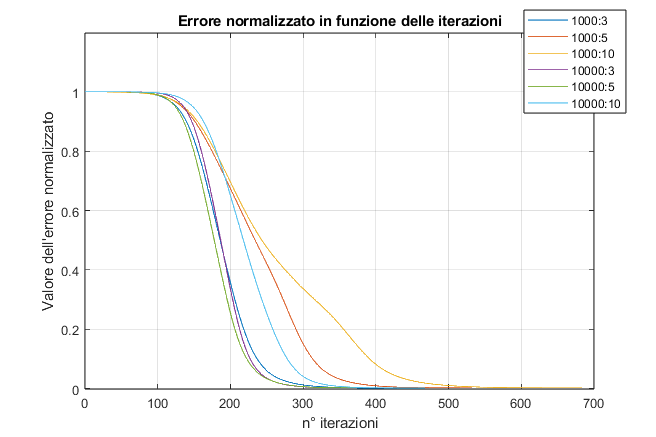
\includegraphics[width=.75\textwidth]{Figures/errors}
\end{figure}
Si può osservare come, al diminuire della complessità campionaria della matrice,
l'algoritmo impieghi meno iterazioni a far convergere l'errore e la funzione
tenda ad assumere una velocità di convergenza geometrica.



\hyphenpenalty=0

\begin{thebibliography}{9}

  \bibitem{8454912}Chi, Y. Low-Rank Matrix Completion [Lecture Notes].
  {\em IEEE Signal Processing Magazine}. \textbf{35}, 178-181 (2018)

\end{thebibliography}
\cleardoublepage\phantomsection % to fix wrong hyperref to \part{Epilogue}

\end{document}
